\documentclass[tikz]{standalone}

\usetikzlibrary{arrows}
\usetikzlibrary{arrows.meta}

\begin{document}


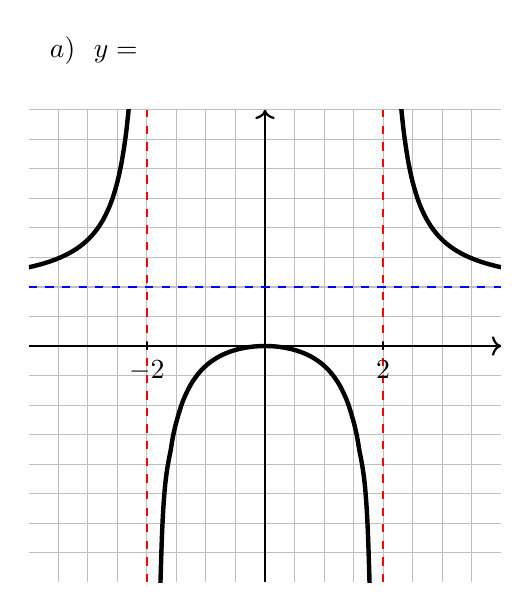
\begin{tikzpicture}[baseline=70,ultra thick,smooth,domain=-4:4,variable=\x,scale=0.75]

    % create a white background with a black frame
    % \draw [thin,fill=white] (-4,-4) rectangle (4,6);  
    
    \node at (-2.9,5) {$a) ~~ y = $};
    
    % draw grid
    \draw[xstep=0.5cm, ystep=0.5cm, lightgray, thin] (-3.99,-3.99) grid (3.99,4); 
    
    % draw axes
    \draw [->,thick] (-4,0) -- (4,0);
    \draw [->,thick] (0,-4) -- (0,4);
    
    
    \clip (-4,-4) rectangle (4,4);
    
    % x^2 / (x^2-4)
    \draw plot [domain=-4:-2.1] (\x,{pow(\x,2) / (\x*\x - 4)}); 
    \draw plot [domain=-1.9:1.9] (\x,{pow(\x,2) / (\x*\x - 4)}); 
    \draw plot [domain=2.1:4] (\x,{pow(\x,2) / (\x*\x - 4)}); 
    
    % asymptotes
    \draw[dashed,red,thick] (-2,-4) -- (-2,4);
    \draw[dashed,red,thick] (2,-4) -- (2,4);
    \draw[dashed,blue,thick] (-4,1) -- (4,1);
    
    % tick marks
    \foreach \x in {-2,2} 
        \draw [thick] (\x cm,2pt) -- (\x cm,-2pt) node[below] {$\x$};
    
\end{tikzpicture}
    
    
    
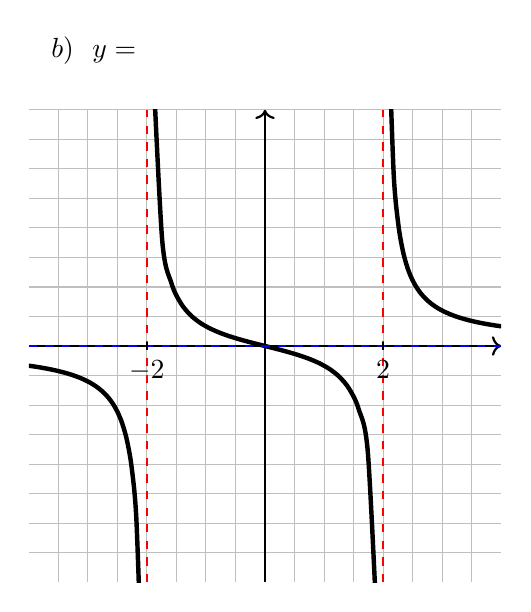
\begin{tikzpicture}[baseline=70,ultra thick,smooth,domain=-4:4,variable=\x,scale=0.75]
    
    % create a white background with a black frame
    % \draw [thin,fill=white] (-4,-4) rectangle (4,6);  
    
    \node at (-2.9,5) {$b) ~~ y = $};
    
    % draw grid
    \draw[xstep=0.5cm, ystep=0.5cm, lightgray, thin] (-3.99,-3.99) grid (3.99,4); 
    
    % draw axes
    \draw [->,thick] (-4,0) -- (4,0);
    \draw [->,thick] (0,-4) -- (0,4);
    
    
    \clip (-4,-4) rectangle (4,4);
    
    % x / (x^2-4)
    \draw plot [domain=-4:-2.1] (\x,{\x / (\x*\x - 4)}); 
    \draw plot [domain=-1.9:1.9] (\x,{\x / (\x*\x - 4)}); 
    \draw plot [domain=2.1:4] (\x,{\x / (\x*\x - 4)}); 
    
    % asymptotes
    \draw[dashed,red,thick] (-2,-4) -- (-2,4);
    \draw[dashed,red,thick] (2,-4) -- (2,4);
    \draw[dashed,blue,thick] (-4,0) -- (4,0);
    
    % tick marks
    \foreach \x in {-2,2} 
        \draw [thick] (\x cm,2pt) -- (\x cm,-2pt) node[below] {$\x$};
    
\end{tikzpicture}
    
    
    
    
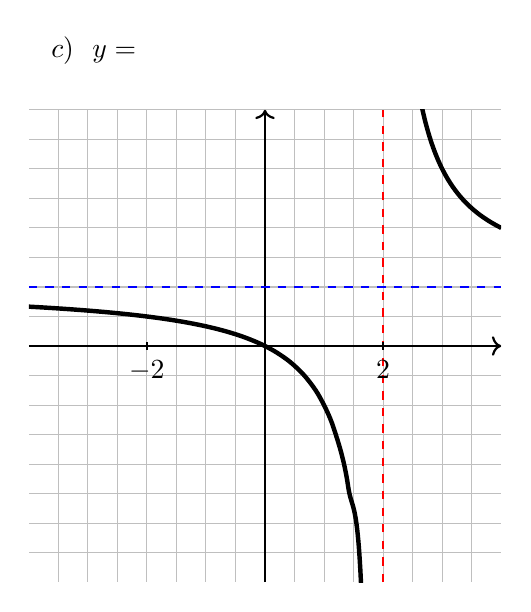
\begin{tikzpicture}[baseline=70,ultra thick,smooth,domain=-4:4,variable=\x,scale=0.75]
    
    % create a white background with a black frame
    % \draw [thin,fill=white] (-4,-4) rectangle (4,6);  
    
    \node at (-2.9,5) {$c) ~~ y = $};
    
    % draw grid
    \draw[xstep=0.5cm, ystep=0.5cm, lightgray, thin] (-3.99,-3.99) grid (3.99,4); 
    
    % draw axes
    \draw [->,thick] (-4,0) -- (4,0);
    \draw [->,thick] (0,-4) -- (0,4);
    
    
    \clip (-4,-4) rectangle (4,4);
    
    % x / (x - 2)
    \draw plot [domain=-4:1.9] (\x,{\x / (\x - 2)}); 
    \draw plot [domain=2.1:4,samples=50] (\x,{\x / (\x - 2)}); 
    
    % asymptotes
    \draw[dashed,red,thick] (2,-4) -- (2,4);
    \draw[dashed,blue,thick] (-4,1) -- (4,1);
    
    % tick marks
    \foreach \x in {-2,2} 
        \draw [thick] (\x cm,2pt) -- (\x cm,-2pt) node[below] {$\x$};
    
\end{tikzpicture}
    
    
    
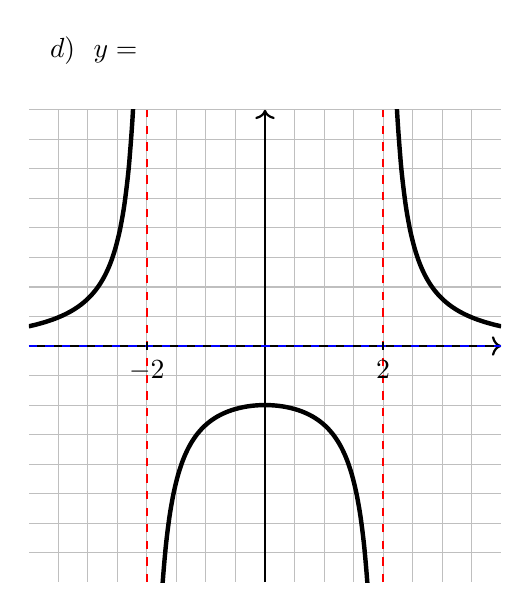
\begin{tikzpicture}[baseline=70,ultra thick,smooth,domain=-4:4,variable=\x,scale=0.75]
    
    % create a white background with a black frame
    % \draw [thin,fill=white] (-4,-4) rectangle (4,6);  
    
    \node at (-2.9,5) {$d) ~~ y = $};
    
    % draw grid
    \draw[xstep=0.5cm, ystep=0.5cm, lightgray, thin] (-3.99,-3.99) grid (3.99,4); 
    
    % draw axes
    \draw [->,thick] (-4,0) -- (4,0);
    \draw [->,thick] (0,-4) -- (0,4);
    
    
    \clip (-4,-4) rectangle (4,4);
    
    % 4 / (x^2-4)
    \draw plot [domain=-4:-2.05] (\x,{4 / (\x*\x - 4)}); 
    \draw plot [domain=-1.95:1.95,samples=60] (\x,{4 / (\x*\x - 4)}); 
    \draw plot [domain=2.05:4] (\x,{4 / (\x*\x - 4)}); 
    
    % asymptotes
    \draw[dashed,red,thick] (-2,-4) -- (-2,4);
    \draw[dashed,red,thick] (2,-4) -- (2,4);
    \draw[dashed,blue,thick] (-4,0) -- (4,0);
    
    % tick marks
    \foreach \x in {-2,2} 
        \draw [thick] (\x cm,2pt) -- (\x cm,-2pt) node[below] {$\x$};
    
    
\end{tikzpicture}

    

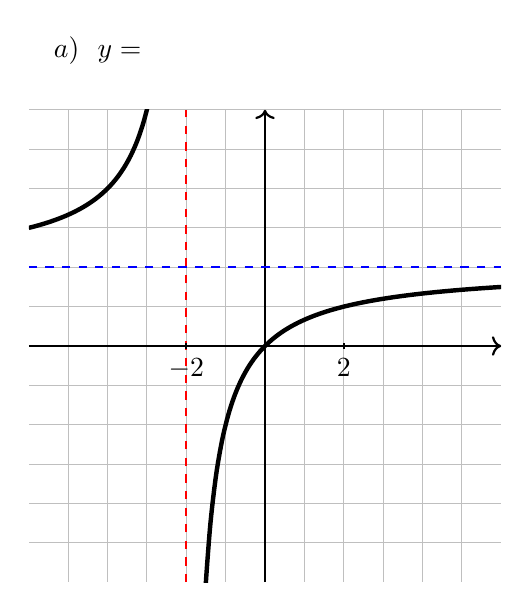
\begin{tikzpicture}[baseline=70,ultra thick,smooth,domain=-6:6,variable=\x,scale=0.5]

    % create a white background with a black frame
    % \draw [thin,fill=white] (-6,-6) rectangle (6,9);  
    
    \node at (-4.25,7.5) {$a) ~~ y = $};
    
    % draw grid
    \draw[xstep=1.0cm, ystep=1.0cm, lightgray, thin] (-5.99,-5.99) grid (5.99,6); 
    
    % draw axes
    \draw [->,thick] (-6,0) -- (6,0);
    \draw [->,thick] (0,-6) -- (0,6);
    
    
    \clip (-6,-6) rectangle (6,6);
    
    % (4x) / (2x+4)
    \draw plot [domain=-6:-2.1] (\x,{(4*\x) / (2*\x + 4)}); 
    \draw plot [domain=-1.9:6,samples=50] (\x,{(4*\x) / (2*\x + 4)}); 
    
    % asymptotes
    \draw[dashed,red,thick] (-2,-6) -- (-2,6);
    \draw[dashed,blue,thick] (-6,2) -- (6,2);
    
    % tick marks
    \foreach \x in {-2,2} 
        \draw [thick] (\x cm,2pt) -- (\x cm,-2pt) node[below] {$\x$};
    
    
\end{tikzpicture}
    
    
    
    
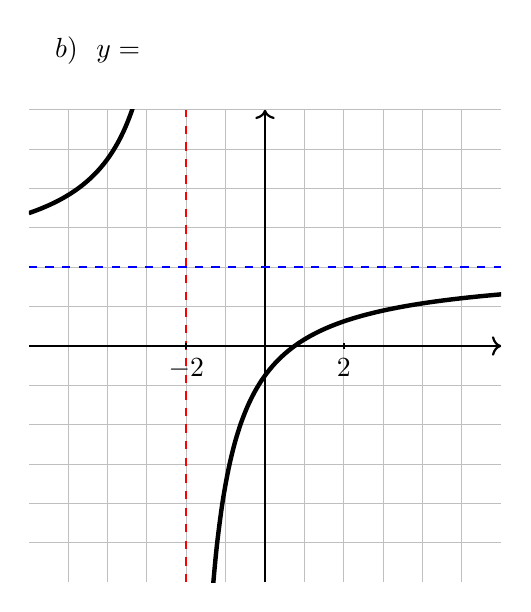
\begin{tikzpicture}[baseline=70,ultra thick,smooth,domain=-6:6,variable=\x,scale=0.5]
    
    % create a white background with a black frame
    % \draw [thin,fill=white] (-6,-6) rectangle (6,9);  
    
    \node at (-4.25,7.5) {$b) ~~ y = $};
    
    % draw grid
    \draw[xstep=1.0cm, ystep=1.0cm, lightgray, thin] (-5.99,-5.99) grid (5.99,6); 
    
    % draw axes
    \draw [->,thick] (-6,0) -- (6,0);
    \draw [->,thick] (0,-6) -- (0,6);
    
    
    \clip (-6,-6) rectangle (6,6);
    
    % (4x-3) / (2x+4)
    \draw plot [domain=-6:-2.1] (\x,{(4*\x - 3) / (2*\x + 4)}); 
    \draw plot [domain=-1.9:6,samples=50] (\x,{(4*\x - 3) / (2*\x + 4)}); 
    
    % asymptotes
    \draw[dashed,red,thick] (-2,-6) -- (-2,6);
    \draw[dashed,blue,thick] (-6,2) -- (6,2);
    
    % tick marks
    \foreach \x in {-2,2} 
        \draw [thick] (\x cm,2pt) -- (\x cm,-2pt) node[below] {$\x$};
    
    
\end{tikzpicture}
    
    
    
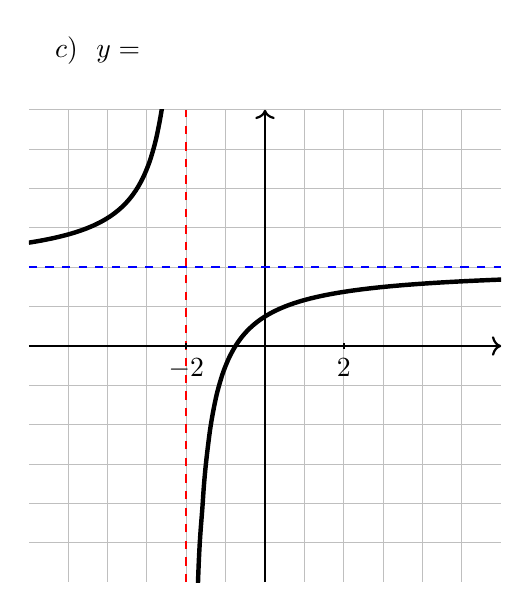
\begin{tikzpicture}[baseline=70,ultra thick,smooth,domain=-6:6,variable=\x,scale=0.5]
    
    % create a white background with a black frame
    % \draw [thin,fill=white] (-6,-6) rectangle (6,9);  
    
    \node at (-4.25,7.5) {$c) ~~ y = $};
    
    % draw grid
    \draw[xstep=1.0cm, ystep=1.0cm, lightgray, thin] (-5.99,-5.99) grid (5.99,6); 
    
    % draw axes
    \draw [->,thick] (-6,0) -- (6,0);
    \draw [->,thick] (0,-6) -- (0,6);
    
    
    \clip (-6,-6) rectangle (6,6);
    
    % (4x+3) / (2x+4)
    \draw plot [domain=-6:-2.1] (\x,{(4*\x + 3) / (2*\x + 4)}); 
    \draw plot [domain=-1.9:6,samples=50] (\x,{(4*\x + 3) / (2*\x + 4)}); 
    
    % asymptotes
    \draw[dashed,red,thick] (-2,-6) -- (-2,6);
    \draw[dashed,blue,thick] (-6,2) -- (6,2);
    
    % tick marks
    \foreach \x in {-2,2} 
        \draw [thick] (\x cm,2pt) -- (\x cm,-2pt) node[below] {$\x$};
    
    
\end{tikzpicture}
    
    
    
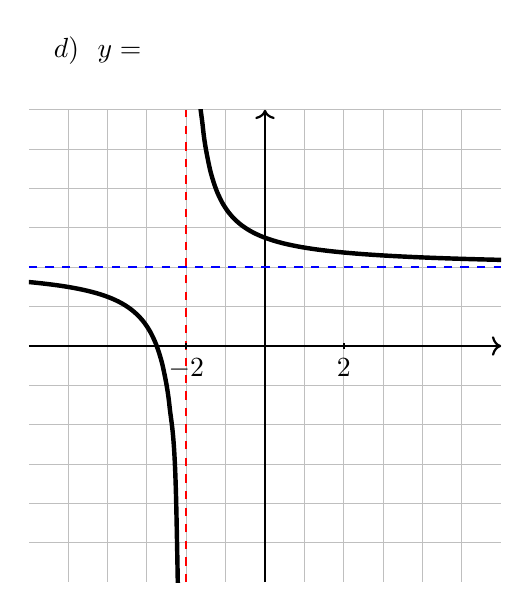
\begin{tikzpicture}[baseline=70,ultra thick,smooth,domain=-6:6,variable=\x,scale=0.5]
    
    % create a white background with a black frame
    % \draw [thin,fill=white] (-6,-6) rectangle (6,9);  
    
    \node at (-4.25,7.5) {$d) ~~ y = $};
    
    % draw grid
    \draw[xstep=1.0cm, ystep=1.0cm, lightgray, thin] (-5.99,-5.99) grid (5.99,6); 
    
    % draw axes
    \draw [->,thick] (-6,0) -- (6,0);
    \draw [->,thick] (0,-6) -- (0,6);
    
    
    \clip (-6,-6) rectangle (6,6);
    
    % (4x+11) / (2x+4)
    \draw plot [domain=-6:-2.1] (\x,{(4*\x + 11) / (2*\x + 4)}); 
    \draw plot [domain=-1.9:6,samples=50] (\x,{(4*\x + 11) / (2*\x + 4)}); 
    
    % asymptotes
    \draw[dashed,red,thick] (-2,-6) -- (-2,6);
    \draw[dashed,blue,thick] (-6,2) -- (6,2);
    
    % tick marks
    \foreach \x in {-2,2} 
        \draw [thick] (\x cm,2pt) -- (\x cm,-2pt) node[below] {$\x$};
    
    
\end{tikzpicture}
    






\end{document} 